\section{Experimental setup and measurement process}
\label{sec:Setup}
For the experimental setup, the Alibava EASy detector system is used. It consists of a control unit, a detector unit
and a computer to control the different measuring modes and for interpreting the taken data. This is done with the
Alibava Graphical User Interface (GUI). The detector and control unit are connected via a ribbon cable, while the 
control unit and the computer are connected via USB. In some measuring tasks, an additional optical fiber cable is
used. In the source measurements, a radioactive source and a LEMO cable for the built-in diode are needed.

\subsection{Detector unit}

The detector unit consists of the semiconductor sensor and readout electronics. A laser system is put on top
of the detector unit, to excite the sensor and trigger signals. The laser system can be put into two different
positions. The "L" position is used for laser measurements and the "Q" position is used for a source measurement
with radioactive material. Triggered signals in the sensor are
amplified in the BEETLE chip and converted into a voltage signal, which can later be interpreted by the control unit.
The signal is kept in a pipeline by the BEETLE chip, until there is an incoming triggering signal from the control unit. Only then will the recorded signal
be passed on to the control unit and computer. If there is no trigger signal, the data is discarded.\\
The depletion voltage of the used semiconductor is usually about $\qty{60}{} -  \qty{70}{\volt}$~\cite{SiliconStrip}. It can be controlled and adjusted
via a knob on the control unit. Knowing the exact depletion voltage will be one of the first measuring tasks, such that the following
tasks can be carried out using the highest efficiency possible. The detecor unit can be seen in \autoref{fig:detector_unit}.
\begin{figure}
    \centering
    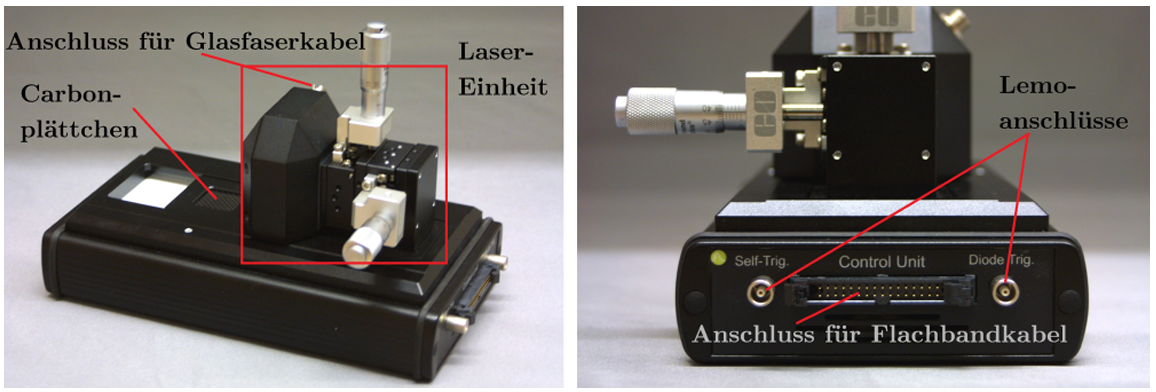
\includegraphics[width = .8\textwidth]{content/pics/detector_unit.png}
    \caption{The detector unit in "Q" position. Top view (left) and side view (right)~\cite{SiliconStrip}.}
    \label{fig:detector_unit}
\end{figure}\\
The used semiconductor sensor consists of a $\qty{300}{\micro\metre}$ thick n-doped silicon layer which is covered by metallisation
on one side. Ohmic resistors are used as a power supply for the sensor. The other side of the silicon layer is covered
by 128 p-doped implants. This creates a pn-semiconductor. The p-doped strip sensors are insulated from each other, so
no current can flow directly between them. This enables a localisation of the incoming signal by reading out which
channel got excited. The strips are then covered by a silicon oxide layer to prevent leakage current to be detected in the readout electronics.
A top-down view and a detailed schematic of the sensor is shown in \autoref{fig:sensor}. The guard ring blocks charge to flow uncontrolled beyond the sensor
and the bias ring supplies the semiconductor with a bias voltage to enlarge the depletion zone. Due to the p-implants
being embedded in the n-base, the semiconductor is called an p-in-n sensor.
\begin{figure}
    \centering
    \begin{subfigure}{0.45\textwidth}
      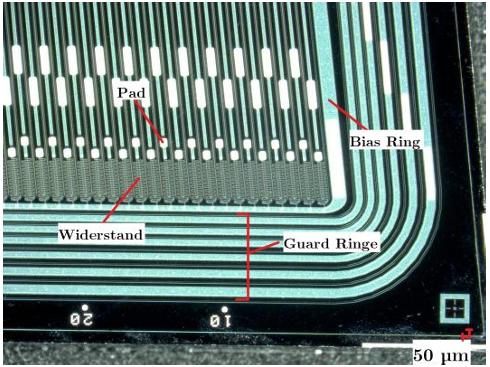
\includegraphics[width = \textwidth]{content/pics/Silicon_Sensor_TOPDOWN.png}
    \end{subfigure}
    \hfill
    \begin{subfigure}{0.45\textwidth}
      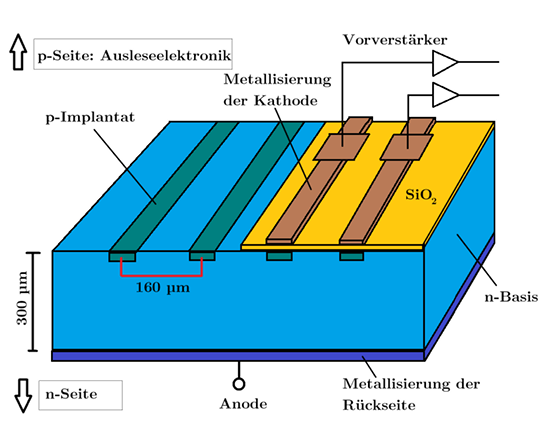
\includegraphics[width = \textwidth]{content/pics/Silicon_Sensor_SCHEMATIC.png}
    \end{subfigure}    
    \caption{Macroscopic top down view (left) and a schematic view of the construction of the whole sensor (right) \cite{SiliconStrip}.}
    \label{fig:sensor}
  \end{figure}\\
The electrons and holes in the n- and p-doped layer recombine if the applied bias voltage is not high enough. If the
bias voltage is applied, an electric field is created such that electrons and holes are seperated. A depletion zone
is caused and gets bigger for higher applied bias voltage. The quality of the sensor can be defined by the charge
collection efficiency (CCE). The higher the applied bias voltage, the bigger the depletion zone and the greater
the CCE gets until a maximum is reached at $U_{\mathrm{dep}}$. This is when the sensor is fully depleted. The CCE can be 
calculated for the applied voltage as
\begin{equation}
    \text{CCE}(U) = \frac{1-\exp{(\frac{-d_c(U)}{a})}}{1-\exp{(\frac{-D}{a})}}.
    \label{eq:CCE}
\end{equation}
$D$ is the thickness of the sensor, $d_c$ is the thickness of the depletion zone and $a$ is the mean penetration depth of
the laser into the silicon. The used sensor has a thickness of $D = \qty{300}{\micro\metre}$. For the source measurement and
therefore the excitation with electrons, the CCE is proportional to $d_c$.\\
The used laser is supplied with energy and controlled via the control unit. A fiber cable transfers the $\qty{5}{\nano\second}$ long laser pulses from
the control unit to the detector unit. The platform has to be in the "L" position for those measurements. It has a 
wavelength of $\qty{980}{\nano\metre}$, a diameter of $\qty{20}{\micro\metre}$ and a peak power of $\qty{0.6}{\milli\watt}$.\\
The horizontal and vertical position of the laser output into the sensor can be adjusted with micrometer screws with an accuracy
of $\qty{10}{\micro\metre}$~\cite{SiliconStrip}.

\subsection{Control unit}

The control unit is used for controlling the laser and the bias voltage of the sensor. It also interprets the taken
data into ADC Counts which can be recorded with the computer. The leakage current is measured with an amperemeter of
the control unit. It can be read out with an accuracy of $\qty{0.01}{\micro\metre}$~\cite{SiliconStrip}.\\
As explained in \autoref{ch:ped}, a lot of noise by the source measurement is also recorded and converted into ADC counts by the detector and control unit.
To distinguish between background and relevant data, a signal-to-noise cut is applied to the data. This signal-to-noise ratio 
can be chosen freely and is set as 5 here. If the signal is five times higher than the noise, it is considered for the analysis.
Otherwise it is discarded.\\
Another source of noise is also the triggering of multiple sensors by only one real signal. This happens, when
a particle passes near the edge of a strip. The created voltage can cause other strips to fire as well. Another effect
would be crosstalk, where a particle crosses perpendicular to the surface and therefore through multiple strips.

\subsection{Measuring tasks}

The measuring tasks in \ref{measure:4} and \ref{measure:5} use the laser. For these tasks, the fibre optic cable
needs to be plugged in into the detector unit and the control unit and the pedestal needs to be in the "L" position.\\
For the measuremets in \ref{measure:5} and \ref{measure:6} the source is used. For this, the detector unit needs
to be put into the box with the source. The detection unit is additionally covered with lead bricks, to prevent radiation to come 
out of the experimental setup. It is still advised not to directly stand over or under the source, since there is no 
lead protection. The pedestal needs to be put into the "Q" position and an additional LEMO cable must be plugged into
the diode trigger of the detector unit and into the control unit. The carbon plate with the source needs to be directly on top
of the sensor. The used setup for the source measurements and the process is shown in \autoref{fig:source_mes}. \\
For the 
source measurements, an additional diode is used, which is placed a few millimetres below the sensor. It ensures, that only
those electrons are regarded, that also triggered a signal in the diode. Only those electrons with enough energy can excite
electron-hole pairs in the sensor and additionally the diode. If the diode triggers a signal, the BEETLE chip switches off
and the signal gets transfered to the control unit.
\begin{figure}
    \centering
    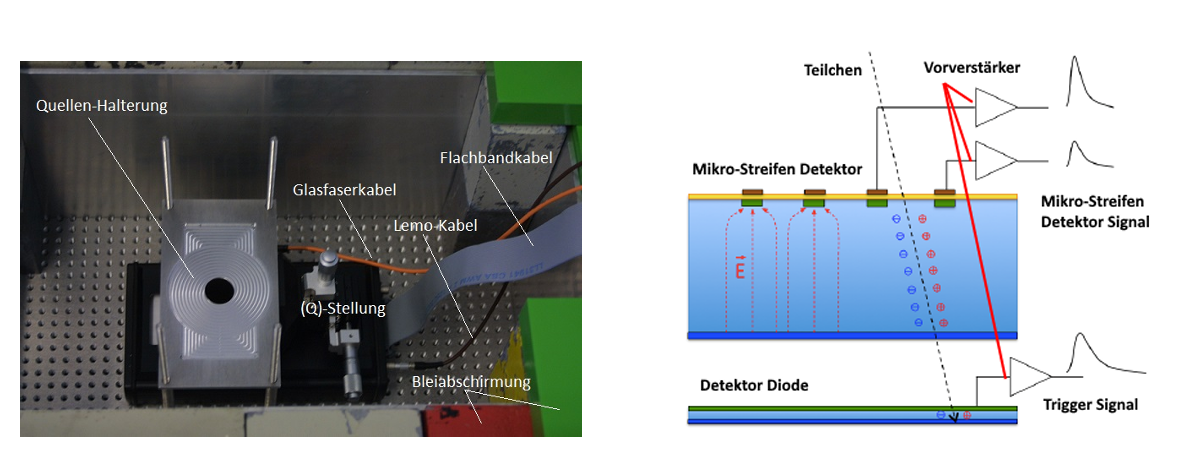
\includegraphics[width = .8\textwidth]{content/pics/Silicon_Sensor_SOURCE.png}
    \caption{Experimental setup for the measurements using the radioactive source (left) and a schematic view of how the sensor
    is triggered with the additional diode (right) \cite{SiliconStrip}.}
    \label{fig:source_mes}
\end{figure}\\

\subsubsection{Current - voltage characteristic}
\label{measure:1}
The current-voltage characteristic is measured by adjusting the bias voltage in $\qty{10}{\volt}$ steps. This way,
the depletion voltage can be extracted. The bias voltage of $\qty{0}{\volt}$ must be carefully set from a higher voltage,
since rotating the knob for the bias to the lowest possible voltage actually applies a voltage in forward direction which causes
the semiconductor to conduct.\\
Use a bias voltage at least $\qty{20}{\volt}$ higher than the estimated depletion voltage for the following measurements.

\subsubsection{Pedestals and noise}
\label{measure:2}
For this measurement, the underlying pedestal is to be measured. To do this, the "Pedestal Run" is chosen in the computer
interface and a run for 1000 events is started. The pedestal and noise for each strip should be plotted and the values of the
common mode represented graphically.

\subsubsection{Calibration measurements}
\label{measure:3}
First, the optimal delay has to be determined. For this, the control unit sends a defined delayed electron pulse to the BEETLE chip,
via the ribbon cable. This is needed to convert the recorded ADC counts into charge and to interpret the data in the following
tasks. The BEETLE chip transmits the measured ADC counts to the control unit. The ADC counts are then plotted against
the used charge. Like this, a calibration curve is obtained which can be used to convert the ADC counts of the following
tasks into charge.\\
To do this, first, a "Delay Measurement" is started. This measures the amount of data obtained for different delays between
the signal and the readout of the signal. The peak of the obtained data series is the best possible delay and is used 
for the following measurements.\\
With the optimal delay applied, calibration measurements for five different channels are started. For a single channel, an additional
measurement for a bias voltage of $\qty{0}{\volt}$ is done.\\
The dependence between the ADC and the charge is to be plotted. The measurement at $\qty{0}{\volt}$ is compared to the other ones above 
the depletion voltage.

\subsubsection{Measuring characterisics of the strip sensors}
\label{measure:4}
In this task, the structure of the sensor strips is to be observed. First, the optimal delay between the laser
and the BEETLE chip is measured by using the "Laser Sync." option in the GUI. With the optimal delay applied, 
35 measurements with each $\qty{1000}{}$ recorded events are carried out. Each measuring point should cover an interval
of $\qty{10}{\micro\metre}$. The signal of relevant strips is to the plotted as a function of the laser position. 
The extension of the laser is to be determined and the number of strips is to be noted.

\subsubsection{Charge Collection Efficiency}
\label{measure:5}
The CCE is measured for both the laser and the source. Since the last measurement included the laser, this setup is used
first. The bias voltage should be increased from $\qty{0}{\volt}$ to $\qty{200}{\volt}$ in $\qty{10}{\volt}$ steps and 
at least $\qty{1000}{}$ events should be recorded for each measuring step. The efficiency of the detector is to be determined
as a function of the bias voltage and the penetration depth of the laser $a$ is to be determined.\\
For the measurement with the source, the detector unit is to be put into the setup for the source measurement and the platform
put into the "Q" position. Again, the bias voltage is increased from $\qty{0}{\volt}$ to $\qty{200}{\volt}$ in $\qty{10}{\volt}$ steps
and at least $\qty{10000}{}$ events should be recorded for each measuring step. The mean cluster energy is to be plotted as a function
of the bias voltage and the results compared to the laser measurement.

\subsubsection{Large source scan}
\label{measure:6}
For the final measurement, the source is to be examined. For this, a RS Run for $\qty{1000000}{}$ events is to be performed.
The data is to be presented graphically is a meaningful way and the number of events per channel should be displayed.
The energy spectrum should be shown in ADC and $\qty{}{\kilo\electronvolt}$ as well. With that, the mean value of the 
deposited energy and the MPV is to be determined and the result evaluated.
